% =============================================================================
%
%                             Theory
%
% =============================================================================
% -----------------------------------------------------------------------------
\chapter{Theoretical Background} \label{chapt:theoreticalback}
% -----------------------------------------------------------------------------
This chapter provides the basics of the project. On the one hand, it is about image processing and filtering as well as communication via Ethernet. What kind of image operations are possible and the Wallis filter are explained in the chapter \ref{chapt:theory:imageprocessing}. An overview of the communication via Ethernet is in the chapter \ref{chapt:theory:ethernet}.


% =============================================================================
%
%                          Image Processing
%
% =============================================================================
\section{Image Processing} \label{chapt:theory:imageprocessing}
In technical terms, image processing is the processing of image data. This includes image processing, image analysis and the output of image files \cite{image_processing}. Procedures that generate a new image can be distinguished into point operations, neighborhood operations and global operations based on their input data. \\
The second part explains the Wallis filter used in this project.

% -----------------------------------------------------------------------------
\subsection{Operations}
% -----------------------------------------------------------------------------
The types of operations that can be applied to images to transform an input image I(u, v) to an output image I'(u, v) can be divided into three categories, which are explained in the following three sections.

\subsubsection*{Point Operations}
The point operations use the color or intensity information at a given pixel in the image as input, calculates a new intensity value as the result and stores it to the same point in the target image (figure \ref{fig:image_operation}a). Typical applications of point operations are, for example, the correction of contrast and brightness, color correction by rotating the color space or the application of different threshold value methods.

Example for a point operation with $u$ and $v$ being pixel coordinates:
\begin{equation}
    I'(u, v) = f(I(u, v))
    \label{eq:point_operation}
\end{equation}


\subsubsection*{Neighborhood Operations} \label{ch:th:neighborhood}
Neighborhood operations use a certain amount of neighboring pixels as input (figure \ref{fig:image_operation}b).
They calculate the result and stored it at the reference point in the target
image. Neighborhood operations are often used in convolution filters. These
filters can be used, for instance, to implement smoothing filters such as the
Gauss filter. Convolution filters can also be used to detect edges in an image. For example, this is possible with the Sobel filter.

Example to calculate the x-derivative and y-derivative with the Sobel matrix \cite{sobel_matrix}:

\noindent\begin{minipage}{.5\linewidth}
\begin{equation}
    G_{x} = I * \begin{bmatrix}
                -1 & 0 & 1 \\ 
                -2 & 0 & 2 \\ 
                -1 & 0 & 1
                \end{bmatrix}
    \label{eq:neighborhood_operation}
\end{equation}

\end{minipage}%
\begin{minipage}{.5\linewidth}

\begin{equation}
    G_{y} = I * \begin{bmatrix}
                -1 & -2 & -1 \\ 
                0 & 0 & 0 \\ 
                1 & 2 & 1
                \end{bmatrix}
    \label{eq:neighborhood_operation}
\end{equation} 

\end{minipage}\\


\textbf{Border Handling:}
With the application of filters, the so-called border handling problem occurs in every image (see figure \ref{fig:image_handling}). Because the filter protrudes beyond the original image.

There are several possible solutions to this issue:
\begin{itemize}
\item The border pixels are not considered. In the example image, the original image 
is two pixels smaller in height and width than the original image. \ref{fig:image_handling}
\item If the filter exceeds the original image, the filter coefficients
at the outside of the image are set to zero
\item The pixels required outside the image are extrapolated according to the closest pixels
\item The image is continued periodically
\end{itemize}
    
\begin{figure}[b!]
    \centering
    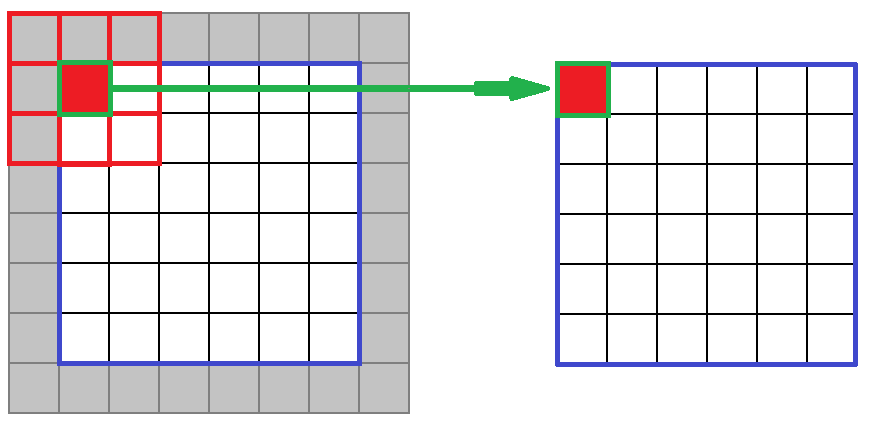
\includegraphics[width=0.6\textwidth]{images/theory/border_handling.png}
    \caption{Border problem with filter operations \cite{border_handling}}
    \label{fig:image_handling}
\end{figure}


\subsubsection*{Global Operations}
Image analysis often employs global image operations that uses the entire image as input data (figure \ref{fig:image_operation}c). It is often about finding regions or recognizing geometrical objects. A typical representative of this is the Hough transform and the Fourier transform.

\begin{figure}[tb!]
    \centering
    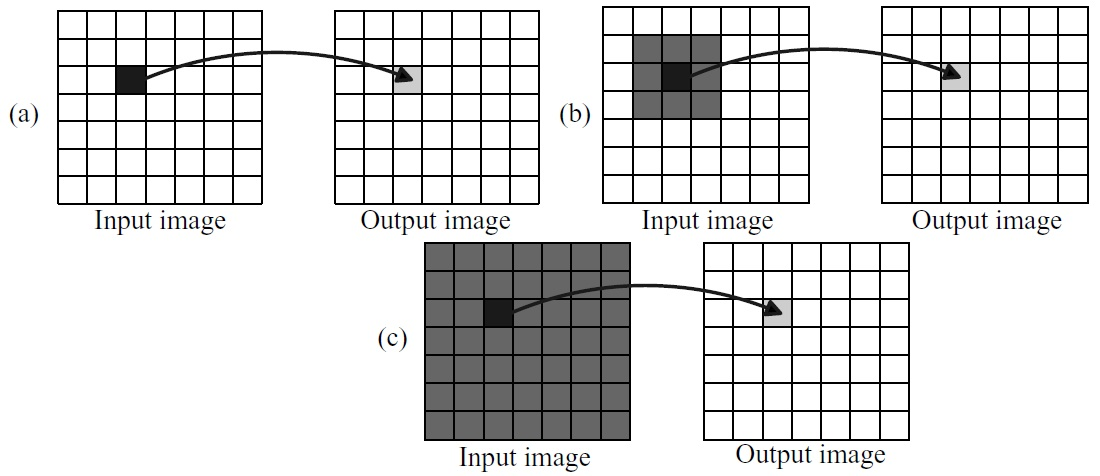
\includegraphics[width=\textwidth]{images/theory/image_operations.jpg}
    \caption{(a) point, (b) neighborhood and (c) global image processing
    operations \cite{image_operation}}
    \label{fig:image_operation}
\end{figure}

% -----------------------------------------------------------------------------
\subsection{Wallis Filter}\label{ch:th_wallis_filter}
% -----------------------------------------------------------------------------
The main goal of the Wallis filter is to adjust the mean and variance of an image and to map it into a given mean and variance to the destination image. This is mainly used for local contrast enhancement in both low and high level regions. It also achieves similair brightness levels in the image.
The Wallis filter equation is \cite{wallis_filter}:
\begin{equation}
    I'(x,y) = \frac{( I(x,y) - \mu_{n})\cdot c \cdot \sigma_{g}^{2}}{c \cdot \sigma_{n}^{2} + (1 - c) \cdot \sigma_{g}^{2}} + b \cdot \mu_{g} + (1 - b) \cdot \mu_{n}
    \label{eq:wallis_filter}
\end{equation} 

\begin{tabular}{rl}
    $I(x,y)         =$ & gray value pixel of the original image \\
    $I'(x,y)        =$ & calculated pixel with the Wallis algorithm \\
    $\mu_{n}        =$ & mean from the neighborhood of the pixel I(x,y) \\
    $\sigma_{n}^{2} =$ & variance from the neighborhood of the pixel I(x,y) \\
    $\mu_{g}        =$ & mean from the destination image \\
    $\sigma_{g}^{2} =$ & variance from the destination image \\
    $b              =$ & brightness factor \\
    $c              =$ & contrast factor \\
\end{tabular} \\

The two facotrs b and c can have the range from 0 to 1. The larger b is selected, the closer it converges to the mean of the desired image $\mu_{g}$. The smaller b is selected, the more it converges to the neighborhood mean $\mu_{n}$.
The bigger the factor c is chosen, the larger is the range of the variance constant $\sigma_{g}^{2}$ \cite{wallis_filter}. \\
The size of the neighborhood depends on the sensor resolution of the camera. The size can be selected from a minimum of 11 to 41 \cite{zeng_2018}. Through the neighborhood operation the smoothing operator is introduced. This means it reduces noise and improves the singal to noise ratio of the image. This in turn enhances image quality \cite{wallis_filter}.


% =============================================================================
%
%                             Ethernet
%
% =============================================================================
\section{Ethernet Communication} \label{chapt:theory:ethernet}
Exchanging data between two devices can be done using different approaches. The
following section contains an overview of the communication standards used in
local area networks (LAN).


\subsection{Open Systems Interconnection (OSI) Model}
Such a telecommunication system can be characterized by the Open Systems 
Interconnection Model. The OSI model is a stack of seven abstraction layers 
grouped into two groups: The host layers and the media layers (see figure \ref{fig:osi}). 
Each layer serves the layer above it and is served with data from the layer
beneath it. In the following chapters the OSI reference model is used to
characterize the Ethernet standard.

\begin{figure}[tb!]
    \centering
    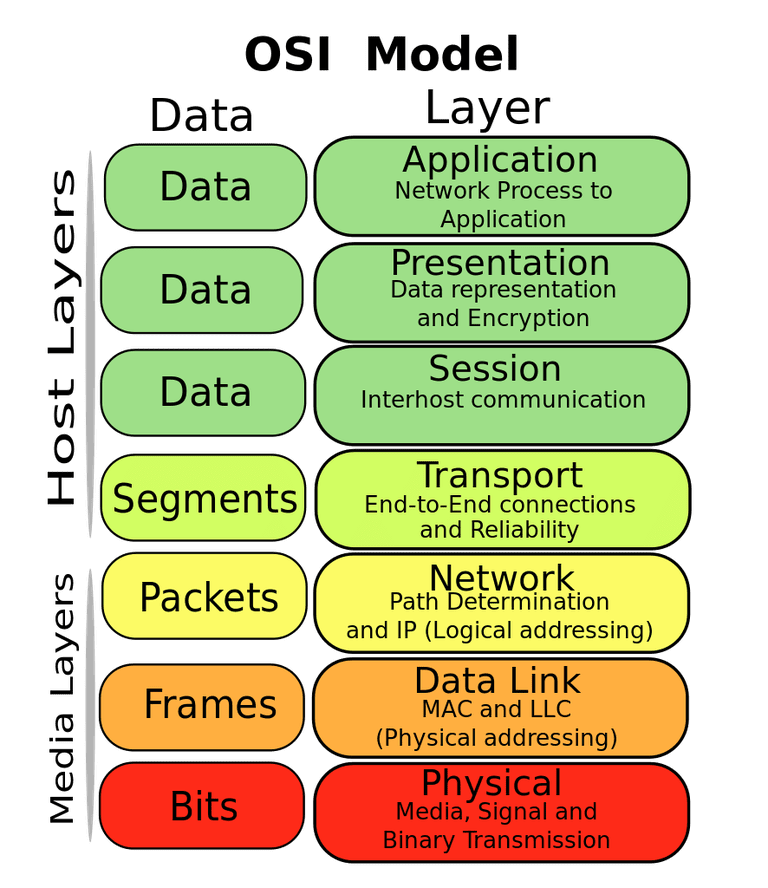
\includegraphics[width=0.5\textwidth]{images/theory/osi.png}
    \caption{OSI Model \cite{osi}}
    \label{fig:osi}
\end{figure}


\subsection{Physical} \label{chapt:theory:physical}
The first layer of the OSI model is the physical layer. It defines the electrical and physical specification of the connection. In the case of local
area networks the connection medium is usually copper. The circuitry required to implement the physical layer is done by the PHY-Chip. This integrated circuit provides digital access through a media independent interface (MII) to the analog physical data link.


\subsection{Data Link} 
The data served from the physical layer is then passed to the data link layer.
Its main purpose is to ensure a reliable transfer of data frames between two
nodes connected by a physical layer. It may also provide means to detect errors
that may occur in the physical layer. Ethernet is the protocol used in the data
layer of local area networks and the layer is split into two sublayers, the logical link control (LLC) and the medium access control (MAC). The LLC provides means to allow multiple network protocols (OSI layer three) to be multiplexed onto the same medium. The MAC encapsulates higher level frames into frames appropriate to be transmitted by the physical layer.
\\

Figure \ref{fig:eth} shows an Ethernet frame. The first seven bytes consist of a fixed preamble. It allows devices on the network to easily synchronize their 
clocks for bit-level synchronization. It is followed by the start frame delimiter (SFD) that marks the beginning of a frame. Sender and receiver MAC addresses ensure that the packet is received by the corresponding host and that it can reply to the sender. The type field indicates the protocol used on the next layer (network layer). After the data payload a frame check sequence in form of a CRC (cyclic redundancy check) is sent to provide error detection. The maximum data payload size is limited to 1500 bytes.
\\

\begin{figure}[tb!]
    \centering
    \begin{adjustbox}{max width=\textwidth}
        \begin{tikzpicture}[
    rounded corners=0mm,
]
    %nodes
    \node[draw, minimum height=1.0cm] (pre) {Preamble};
    \node[draw, minimum height=1.0cm, right = 0cm of pre] (sfd) {SFD};
    \node[draw, minimum height=1.0cm, right = 0cm of sfd] (dst) {Destination MAC Adr.};
    \node[draw, minimum height=1.0cm, right = 0cm of dst] (src) {Source MAC Adr.};
    \node[draw, align = center, text width=1cm, minimum height=1.0cm, right = 0cm of src] (tp) {Type\\Field};
    \node[draw, minimum height=1.0cm, right = 0cm of tp] (dat) {Data (46 - 1500 Bytes)};
    \node[draw, minimum height=1.0cm, right = 0cm of dat] (pad) {PAD};
    \node[draw, minimum height=1.0cm, right = 0cm of pad] (crc) {CRC};

    \path[draw,-] ($(dst.180) + (0,0)$) -- ++(0,1.2) ;
    \path[draw,-] ($(crc.0) + (0,0)$) -- ++(0,1.2) ;
    \path[draw,{Latex[length=2.5mm]}-{Latex[length=2.5mm]}] ($(dst.180) + (0,1.0)$) -- ($(crc.0) + (0,1.0)$) node [midway, above] () {Basic MAC Frame} ;
\end{tikzpicture}
    \end{adjustbox}
    \caption{Ethernet Frame}
    \label{fig:eth}
\end{figure}
The medium access controller is implemented in hardware to ensure that every bit is received and stored. The transmit and receive data is commonly stored in
FiFo (first in first out) buffers. This way the next layer in the OSI model is
not required to have low latency capability.


\subsection{Network} 
The data link layer provides means to send frames across nodes in the same
network. As soon as the destination node is in another network, a network layer
is required. Using logical device addresses, network packets can be routed
across different networks and on different media. This allows data to be sent
over long distances.
\\

The most commonly used network layer is the Internet Protocol version 4 (IPv4).
It consists of a 20 byte sized header that contains destination and source IP
addresses, total length, checksum and other fields. The protocol field indicates what layer four protocol is used. Figure \ref{fig:ip} shows a complete IPv4 header.

\begin{figure}[tb!]
    \centering
    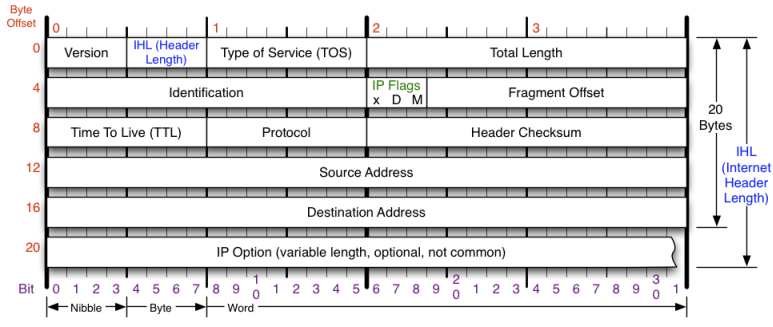
\includegraphics[width=\textwidth]{images/theory/ip.png}
    \caption{IPv4 header \cite{ip}}
    \label{fig:ip}
\end{figure}
\begin{figure}[tb!]
    \centering
    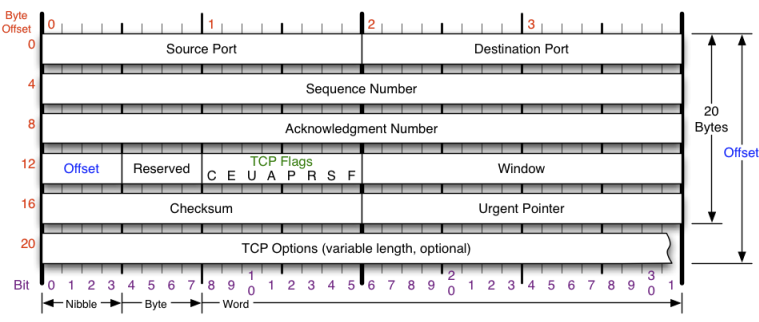
\includegraphics[width=\textwidth]{images/theory/tcp.png}
    \caption{TCP Header \cite{tcpudp}}
    \label{fig:tcp}
\end{figure}
\begin{figure}[tb!]
    \centering
    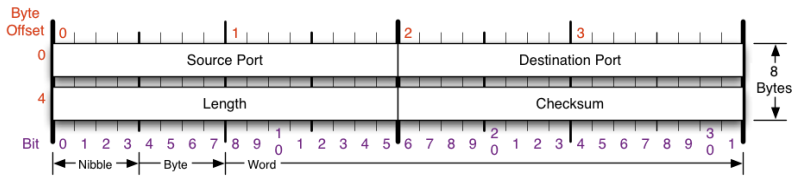
\includegraphics[width=\textwidth]{images/theory/udp.png}
    \caption{UDP Header \cite{tcpudp}}
    \label{fig:udp}
\end{figure}


\subsection{Transport} 
The transport layer is the first layer in the OSI model that is not required by
the network. Its main purpose is to control the communication of different
applications on two hosts. Therefore a port number is required to distinguish
between the different applications utilizing the same network connection. The
transport layer may also provide segmentation of the data, guarantee of delivery and flow control to avoid network jam.
\\

The two most used transport layer protocols are the Transmission Control
Protocol (TCP) and the User Datagram Protocol (UDP). Table \ref{tab:tcpudp}
shows the main differences between these two protocols. The most important
aspect is the protocol connection setup. While UDP is connection less (data is
sent without setup), TCP establishes a connection between host and client
prior to data transmission. This ensures a reliable data delivery hence all
messages are acknowledged. UDP has its benefits in lower overhead and for that
reason has slightly higher transmission speed but the protocol does not
guarantee that the message has been received by the client.

\begin{table}[h]
    \centering
    \begin{tabular}{ l  c  c }
        \toprule
         & \textbf{TCP} & \textbf{UDP} \\
        \midrule
        Connection oriented & Yes & No \\
        Header size & 20 Byte & 8 Byte \\
        Reliable transmission & Yes & No \\
        Acknowledge & Yes & No \\
        Segmentation & Yes & No \\
        Best for & reliable transfer & fast transfer  \\
        \bottomrule
    \end{tabular}
    \caption{TCP vs. UDP}
    \label{tab:tcpudp}
\end{table}

\section{Vivado HLS} \label{ch:th:hls}
Vivado HLS is a development environment that synthesizes C/C++ code in VHDL. The C/C++ language is intended for sequential programming where the VHDL language describes the hardware. This chapter deals with the design flow (\ref{ch:design_flow})of Vivado HLS. The directives (\ref{ch:directives}) that are for the compiler to synthesize the C/C++ code in VHDL and finally arbritary data types (\ref{ch:ap}). Which can be used in the Vivado HLS for C/C++ code.

\subsection{Design Flow} \label{ch:design_flow}
In Vivado HLS it is possible to translate the C/C++ code into VHDL and generate an IP core for Vivado HLx. To ensure that the algorithm is correct, it can be validated in various steps. These steps are the design flow of Vivado HLS and are shown in figure \ref{fig:hls_design_flow}.
First of all, the C/C++ algorithm can be tested in a simulation. This requires a testbench in addition to the C/C++ algorithm. As soon as the algorithm works satisfyingly the design can be run through synthesis and generating a RTL design in VHDL. VHDL design can be verified in an RTL simulation. The RTL simulation must match the C/C++ simulation. If this is the case, an IP core can be generated from the VHDL code and used in the Vivado HLx \cite{vivado_hls}.

\begin{figure}[tb!]
    \centering
    % \tikzsetnextfilename{system-overview}
\begin{tikzpicture}[
    rounded corners=0mm,
]
    %coordinates
    \coordinate (orig)      at (0,0);
    \coordinate (test)      at (-3,0);
    \coordinate (alg)       at (3,0);
    \coordinate (c_sim)     at (0,-1);
    \coordinate (c_synth)   at (0,-2);
    \coordinate (VHDL)      at (0,-3);
    \coordinate (rtl_sim)   at (0,-4);
    \coordinate (ip)        at (0,-5);
    \coordinate (hlx)       at (0,-6);

    %nodes
    \node[draw, fill=white, minimum width=4cm, minimum height=0.6cm, anchor=south, text width=3.8cm, align=center, rounded corners=3mm] (A) at (test) {C/C++ Testbench};
    \node[draw, fill=white, minimum width=4cm, minimum height=0.6cm, anchor=south, text width=3.8cm, align=center, rounded corners=3mm] (B) at (alg) {C/C++ Algorithm};
    \node[draw, fill=white, minimum width=4cm, minimum height=0.6cm, anchor=south, text width=3.8cm, align=center] (C) at (c_sim) {C/C++ Simulation};
    \node[draw, fill=white, minimum width=4cm, minimum height=0.6cm, anchor=south, text width=3.8cm, align=center] (D) at (c_synth) {C/C++ Synthesis};
    \node[draw, fill=white, minimum width=4cm, minimum height=0.6cm, anchor=south, text width=3.8cm, align=center, rounded corners=3mm] (E) at (VHDL) {VHDL};
    \node[draw, fill=white, minimum width=4cm, minimum height=0.6cm, anchor=south, text width=3.8cm, align=center] (F) at (rtl_sim) {RTL Simulation};
    \node[draw, fill=white, minimum width=4cm, minimum height=0.6cm, anchor=south, text width=3.8cm, align=center] (G) at (ip) {Package IP};
    \node[draw, fill=white, minimum width=4cm, minimum height=0.6cm, anchor=south, text width=3.8cm, align=center] (H) at (hlx) {Vivado HLx};

    %path
    \path [draw,-] (A) -- (B);
    \path[draw,-{Latex[length=2.5mm]}] (A) -| (C);
    \path[draw,-{Latex[length=2.5mm]}] (C.east) -- ++(3.5,0) |- (B.east);
    \path[draw,-{Latex[length=2.5mm]}] (C) -- (D);
    \path[draw,-{Latex[length=2.5mm]}] (D) -- (E);
    \path[draw,-{Latex[length=2.5mm]}] (E) -- (F);
    \path[draw,-{Latex[length=2.5mm]}] (E.west) -- ++(-0.5,0) |- (G.west);
    \path[draw,-{Latex[length=2.5mm]}] (F.east) -- ++(3.5,0) |- (B.east);
    \path[draw,-{Latex[length=2.5mm]}] (G) -- (H);


\end{tikzpicture}
    \caption{Vivado HLS design flow}
    \label{fig:hls_design_flow}
\end{figure}

\subsection{Directives} \label{ch:directives}
If the FPGA is programmed using C/C++ language, there is no way to get around the directives. Directives are instructions to the compiler on how it should synthesize and optimize the code. Latency, throughput or area can be optimized \cite{pragma}. The following three chapters explain some important directives to reduce the latency and increase the throughput. \\
Directives are also called pragmas and can be written directly into the C/C++ code or added as directives in a separate tcl-file.

\todo[inline]{Bilder von Interfce, Array Partition und Pipeline / Unroll anpassen!}

\subsubsection*{Interface}
The directive \texttt{interface} specifies the input and output ports of the IP core. Different interfaces can be implemented in the IP core as input and output ports. Among others, these are control interfaces or interfaces for data. \\
The IP core can be controlled with the control interfaces. With this signal it can be started or stopped for example or send a handshake if the IP core has the operation finished. \\
AXI4 interfaces can also be added directly to the IP core by directives. The AX4-Lite, AXI4-Master or AXI4-Stream interface can be connected. \\
Among other things, memory elements can also be connected directly to the IP core. These are block RAM or FIFOs that can be used to read and process the data with the IP core. These can also be used to store output data of the IP core \cite{pragma}. \\
The figure \ref{fig:p_interface} shows how the pragma \texttt{interface} is configured. First, the interface can be specified and whether it is an input or an output. Finally, the variable to which the pragma is to be applied.

\begin{figure}[tb!]
    \centering
    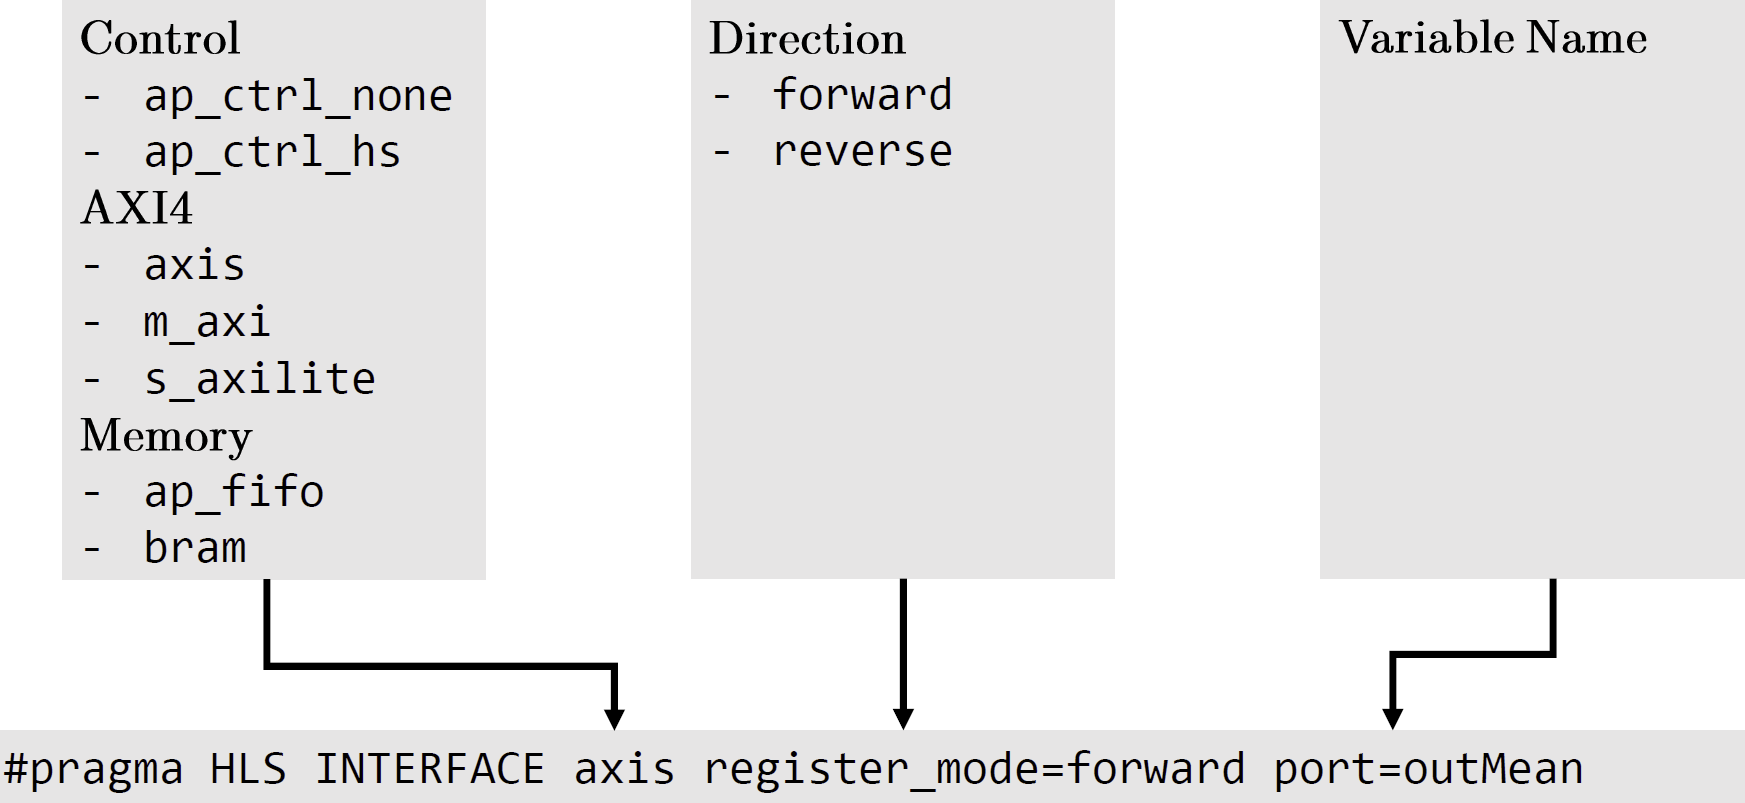
\includegraphics[width=\textwidth]{images/theory/interface.png}
    \caption{Pragma: interface}
    \label{fig:p_interface}
\end{figure}

\subsubsection*{Array Partition}
The \texttt{array\_partition} directive splits an array into several smaller elements. This means that in RTL synthesis several smaller memories or registers are used from a larger memory. However, this increases the throughput in the design but also the read and write ports for the storage. \\
The figure \ref{fig:p_array_partition} shows the three different methods of partitioning an array.

\begin{description}
\item[Block]\hfill \\
The whole array is split into several arrays of the same size. The elements are stored in the same order as in the array. The array is simply cropped apart.
\item[Cyclic]\hfill \\ 
The array is split into equal parts like \texttt{block}, but the storage order is different. As can be seen, each following element is stored in a different memory. 
\item[Complete]\hfill \\ 
This argument splits the complete array into individual elements.
\end{description}


\begin{figure}[tb!]
    \centering
    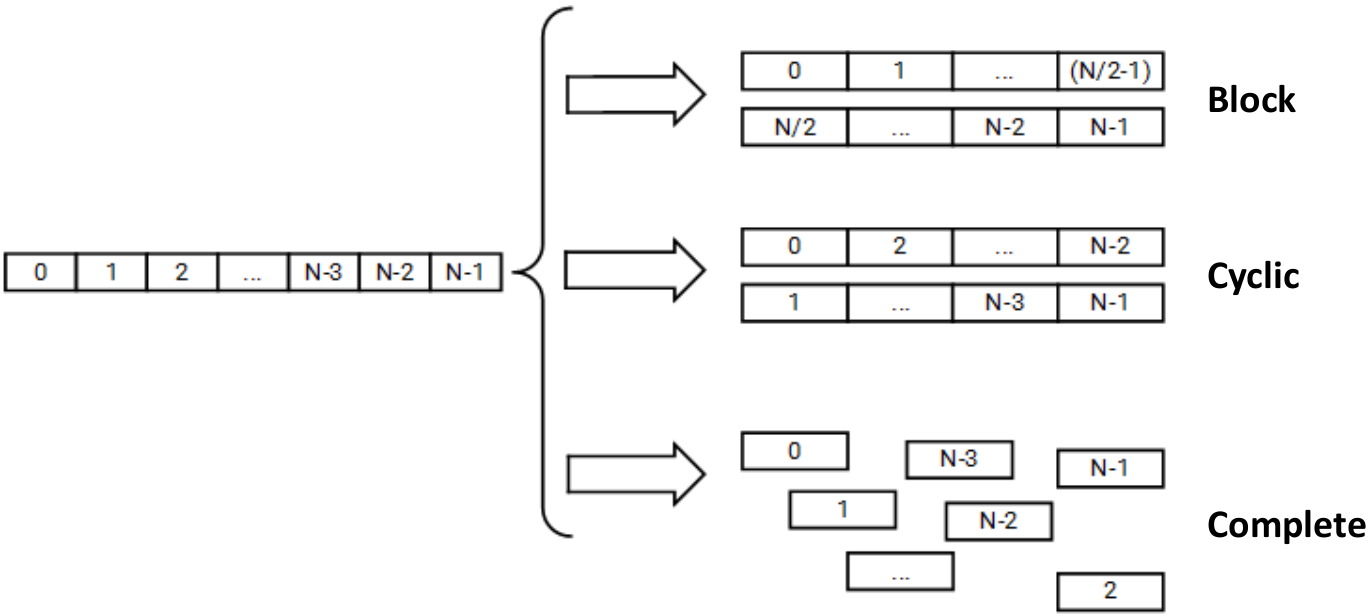
\includegraphics[width=\textwidth]{images/theory/array_partition.png}
    \caption{Pragma: array\_partition}
    \label{fig:p_array_partition}
\end{figure}

\subsubsection*{Pipeline / Unroll}
In Vivado HLS the FPGA is described with C/C++ language. Among others, it is also possible to program for loops. These are still processed sequentially by the RTL synthesis, as can be seen in the figure \ref{fig:p_pipeline_unroll} with 9 clock cycles. The directive can improve the performance of the for loop. Two directives are available to increase the throughput of a for loop. These are \texttt{pipeline} and \texttt{unroll}.

\begin{description}
\item[Pipeline]\hfill \\
This directive allows a for loop to be parallelized. This increases the throughput and the area. Now that more operations are happening in a clock.
Pipeline is used if not all data for processing is available in the for loop. The figure \ref{fig:p_pipeline_unroll} shows that the read access leads to a latency of one clock cycle and the throughput could be increased.
\item[Unroll]\hfill \\ 
This directive allows the for loop to be fully parallelized. This is only possible if all the data that is required in the for loop is available. The figure \ref{fig:p_pipeline_unroll} shows that the entire for loop is now processed in one cycle. This again leads to an increase in throughput and the area in relation to directive \texttt{pipeline}.
\end{description}

With nested for loops, note that if pipeline is applied to the top loop, the inner for loops are automatically unrolled. \\
You can also apply both directives in combination in a for loop. Since the unroll directive can specify a factor that unrolls the loop.

\begin{figure}[tb!]
    \centering
    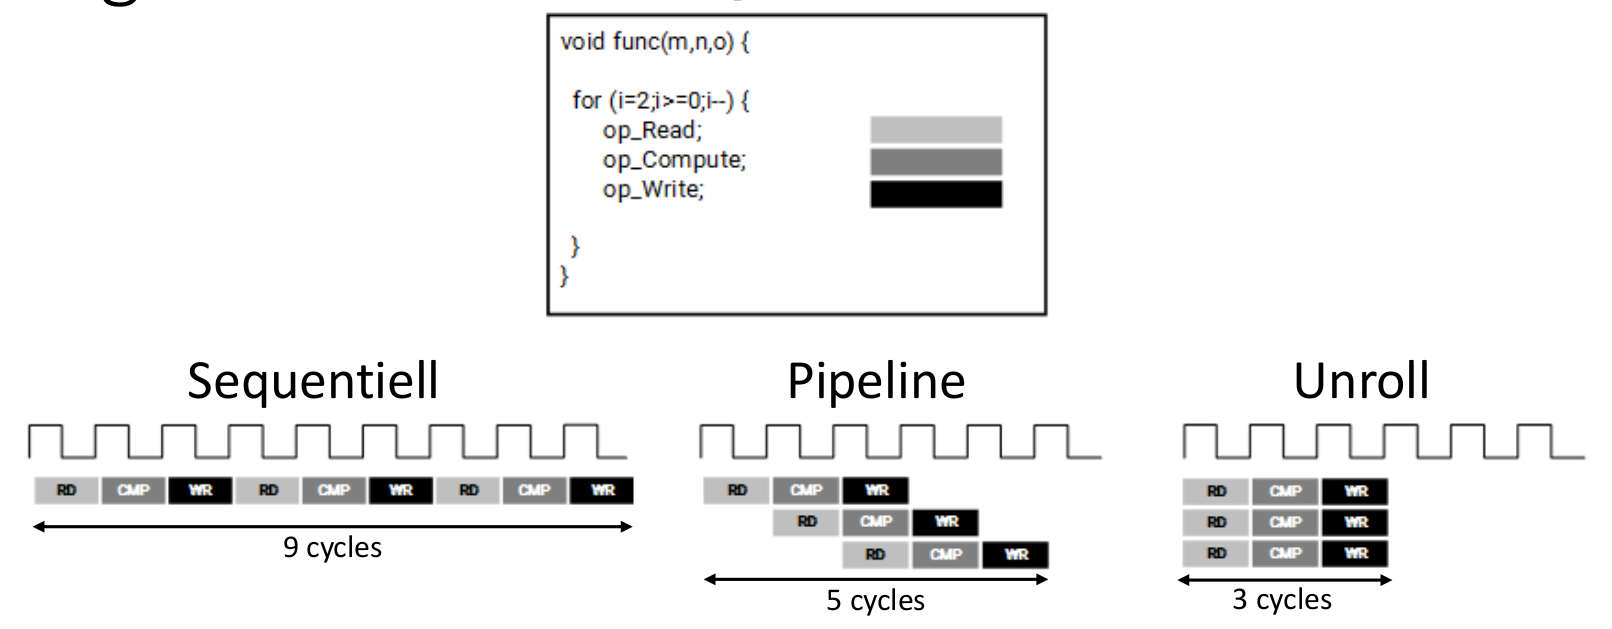
\includegraphics[width=\textwidth]{images/theory/pipeline_unroll.png}
    \caption{Pragma: pipeline / unroll}
    \label{fig:p_pipeline_unroll}
\end{figure}

\subsection{Arbitrary Precision} \label{ch:ap}
Resources are limited in the FPGA. Therefore it is often a big waste of resources when calculating with too large data types or even floating point in the FPGA \cite{floating}. Viviado HLS supports arbitrary precision data types using C/C++ code. With this it is possible to counteract the problem of large data types and floating point. \\

\textbf{Arbitrary Precision Integer:}
Arbitrary Precision Integers are data types where it is possible to define any bit width. This has the advantage that resources can be reduced. Because it is not necessary to select the data types provided in C/C++ (8, 16, 32 bit or char, short, int etc.) \\
To use these data types only the header file \texttt{ap\_int.h} must be included. The following example shows how a 11 bit signed integer and a 5 bit unsigned integer be defined \cite{ug902}.

\begin{minipage}{\textwidth}
\begin{lstlisting}[style=CStyle]
ap_int<11> var1;
ap_uint<5> var2;
\end{lstlisting}
\end{minipage} \\

\textbf{Arbitrary Precision Fixed-Point:}
Floating Point can be used on the FPGA, but this usually requires a lot of resources. Viviado HLS has a library for Arbitrary Precision Fixed Point data types, which can be used to calculate sufficiently accurate. With these fixed point data types many resources can be saved. \\
For this purpose there is the library \texttt{ap\_fixed.h} and must be included. The data types are defined so that the first number represents the whole data type width and the second number represents the above number of the binary point. The following example shows an unsigned 11 bit varibale with 3 bits representing the integer value and 8 bits representing the fractional value \cite{ug902}. 

\begin{minipage}{\textwidth}
\begin{lstlisting}[style=CStyle]
ap_ufixed<11,3> fp_var;
\end{lstlisting}
\end{minipage}
